\chapter{Mathematical Circuits Using Op.Amp.: Part II}


\section{Objectives}
\begin{itemize}
    \item To verify Op.Amp. circuits for differentiation operation
    \item To verify Op.Amp. circuits for integration operation
    \item To verify Op.Amp. circuits for logarithm operation
    \item To verify Op.Amp. circuits for exponentiation operation
\end{itemize}

\section{Materials}
\begin{itemize}
    \item Breadboard
    \item Capacitors
    \item DC power supply
    \item Digital Multi-Meter
    \item \hyperref[1N4148]{Diode (1N4148)}
    \item Function Generator
    \item \hyperref[LM741_1]{Op.Amp. (LM741)}
    \item Oscilloscope
    \item Resistors
\end{itemize}

\section{Introduction}
    \subsection{Circuit Diagram}
    \begin{figure}[h]

        \begin{subfigure}[h]{0.47\textwidth}
        \begin{center}
            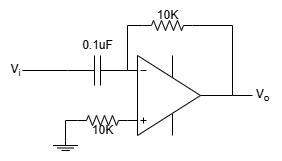
\includegraphics[width=1\linewidth]{Lab11/Lab11a.drawio.png}
            \caption{}
            \label{L11a}
        \end{center} 
        \end{subfigure}
    \hfill
    \vspace{0.2 cm}
        \begin{subfigure}[h]{0.47\textwidth}
        \begin{center}
            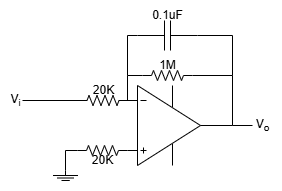
\includegraphics[width=1\linewidth]{Lab11/Lab11b.drawio.png}
            \caption{}
            \label{L11b}
        \end{center}
        \end{subfigure}
    \vfill
    
    \vspace{0.2 cm}
        \begin{subfigure}[h]{0.47\textwidth}
        \begin{center}
            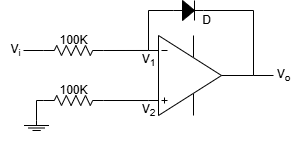
\includegraphics[width=1\linewidth]{Lab11/Lab11c.drawio.png} 
            \caption{}
            \label{L11c}
        \end{center}
        \end{subfigure}
    \hfill
        \begin{subfigure}[h]{0.47\textwidth}
        \begin{center}
            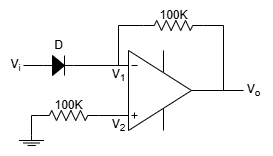
\includegraphics[width=1\linewidth]{Lab11/Lab11d.drawio.png}
            \caption{}
            \label{L11d}
        \end{center}
        \end{subfigure}

    \caption{Different fundamental Op.Amp. circuits}
    \label{l11fs}
    
    \end{figure}
    \FloatBarrier

\section{Detailed Procedures}
    \subsection{Analyzation}
    In this experiment, because it is not all the resistor's resistance can meet the requirement on the figures, some of the resistors are combined resistors, therefore for the accuracy all the components were measured, with the values of:
    \begin{itemize}
        \item 20K: 20.01K
        \item 10K: 9.775K
        \item 100K: 99.19K
        \item 6.2K: 6.218K
        \item 12K: 11.77K
        \item 18.2K: 18.0K\~18.11K
    \end{itemize}
    \begin{itemize}
        \item 20K: 20.01K
        \item 10K: 9.775K
        \item 100K: 99.19K
        \item 6.2K: 6.218K
        \item 12K: 11.77K
        \item 18.2K: 18.0K\~18.11K
    \end{itemize}
    \begin{itemize}
        \item For Fig.\ref{L11a},
            \begin{equation}
                V_o=-10K\cdot0.1\mu\frac{dV_i}{dt}
            \end{equation}
        \item For Fig.\ref{L11b},
            \begin{equation}
                V_o=-\frac{1}{20K\times0.1\mu}\int V_i \,dt
            \end{equation}
        \item For Fig.\ref{L11c},
            \begin{equation}
                \begin{cases}
                    V_o=-V_\gamma & V_i<0,~\text{D off}\\
                    V_o=nV_Tln(\frac{V_i}{I_S-100K}) & V_i>0,~\text{D on}\\
                \end{cases}
            \end{equation}
        \item For Fig.\ref{L11d},
            \begin{equation}
                V_o=-100KI_Se^{-\frac{V_i}{nV_T}}
            \end{equation}
    \end{itemize}
    
    \subsection{Procedures}
    \begin{itemize}
        \item For Fig.\ref{L11a},\\
        With sinusoidal signal input:\\
\begin{table}[h]
\centering
\begin{tabular}{|ccc|ccc|}
\hline
\multicolumn{3}{|c|}{Vi=1V}                                       & \multicolumn{3}{c|}{Vi=2V}                                      \\ \hline
\multicolumn{1}{|c|}{$f$} & \multicolumn{1}{c|}{Amp(m)} & $\phi$  & \multicolumn{1}{c|}{$f$} & \multicolumn{1}{c|}{Amp(m)} & $\phi$ \\ \hline
\multicolumn{1}{|c|}{50}  & \multicolumn{1}{c|}{185}    & -104.16 & \multicolumn{1}{c|}{200} & \multicolumn{1}{c|}{180}    & 94.56  \\ \hline
\multicolumn{1}{|c|}{100} & \multicolumn{1}{c|}{93.5}   & -93.37  & \multicolumn{1}{c|}{400} & \multicolumn{1}{c|}{290}    & 94.4   \\ \hline
\multicolumn{1}{|c|}{150} & \multicolumn{1}{c|}{61.5}   & -88.7   & \multicolumn{1}{c|}{600} & \multicolumn{1}{c|}{420}    & 91.53  \\ \hline
\multicolumn{1}{|c|}{200} & \multicolumn{1}{c|}{47}     & -89.93  & \multicolumn{1}{c|}{800} & \multicolumn{1}{c|}{545}    & 96.43  \\ \hline
\multicolumn{1}{|c|}{}    & \multicolumn{1}{c|}{}       &         & \multicolumn{1}{c|}{1K}  & \multicolumn{1}{c|}{665}    & 97.49  \\ \hline
\end{tabular}
\end{table}
\FloatBarrier
    With square signal input:\\
    \begin{figure}[h]
        \centering
        \includegraphics[width=0.5\linewidth]{Lab11/l11asqwf.png}
        \caption{Square Signal}
        \label{l11asqwf}
    \end{figure}
\FloatBarrier
An output signal is generated only when the edge of the input signal changes direction along the x-axis. This behavior is attributed to the presence of the capacitor in the circuit. Capacitors allow only alternating signals to pass through while blocking direct current (DC) or constant signals. Meanwhile, a square wave signal behaves as a DC signal when its polarity remains unchanged.

        \item For Fig.\ref{L11b},\\
\begin{table}[h]
\centering
\begin{tabular}{|ccc|}
\hline
\multicolumn{3}{|c|}{Vi=1V}                                      \\ \hline
\multicolumn{1}{|c|}{$f$} & \multicolumn{1}{c|}{Amp(m)} & $\phi$ \\ \hline
\multicolumn{1}{|c|}{50}  & \multicolumn{1}{c|}{3.25}   & -90.92 \\ \hline
\multicolumn{1}{|c|}{100} & \multicolumn{1}{c|}{1.55}   & -90.01 \\ \hline
\multicolumn{1}{|c|}{150} & \multicolumn{1}{c|}{1.03}   & -89.30 \\ \hline
\multicolumn{1}{|c|}{200} & \multicolumn{1}{c|}{0.83}   & -89.71 \\ \hline
\end{tabular}
\end{table}

        \item For Fig.\ref{L11c},\\
\begin{figure}[h]
    \centering
    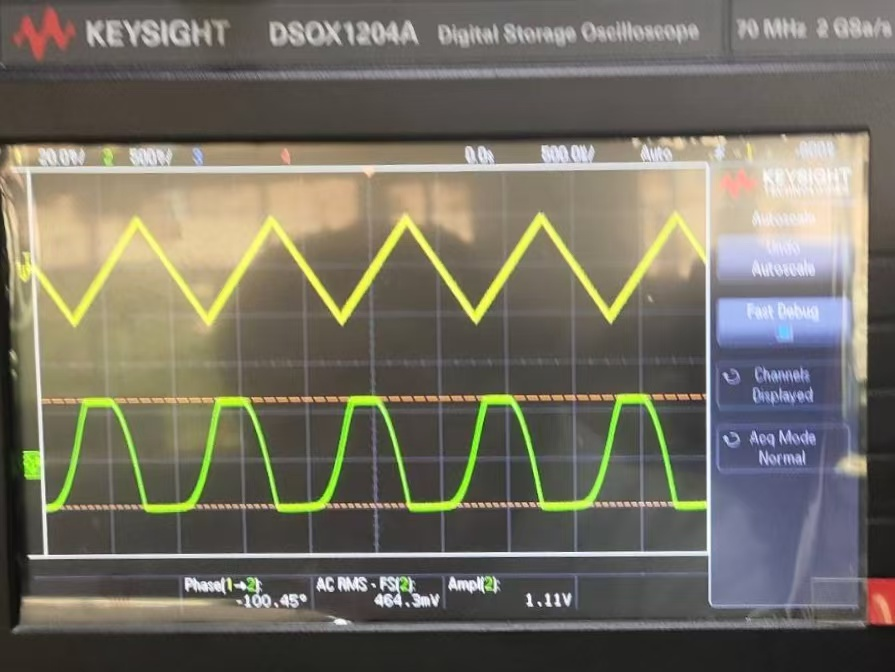
\includegraphics[width=0.5\linewidth]{Lab11/l11cwf.jpg}
    \caption{Wavefrom}
    \label{fig:enter-label}
\end{figure}
\FloatBarrier
        The amplitude of $v_i$ we adjusted is 0.020V. 
        \item For Fig.\ref{L11d},\\
\begin{figure}[h]
    \centering
    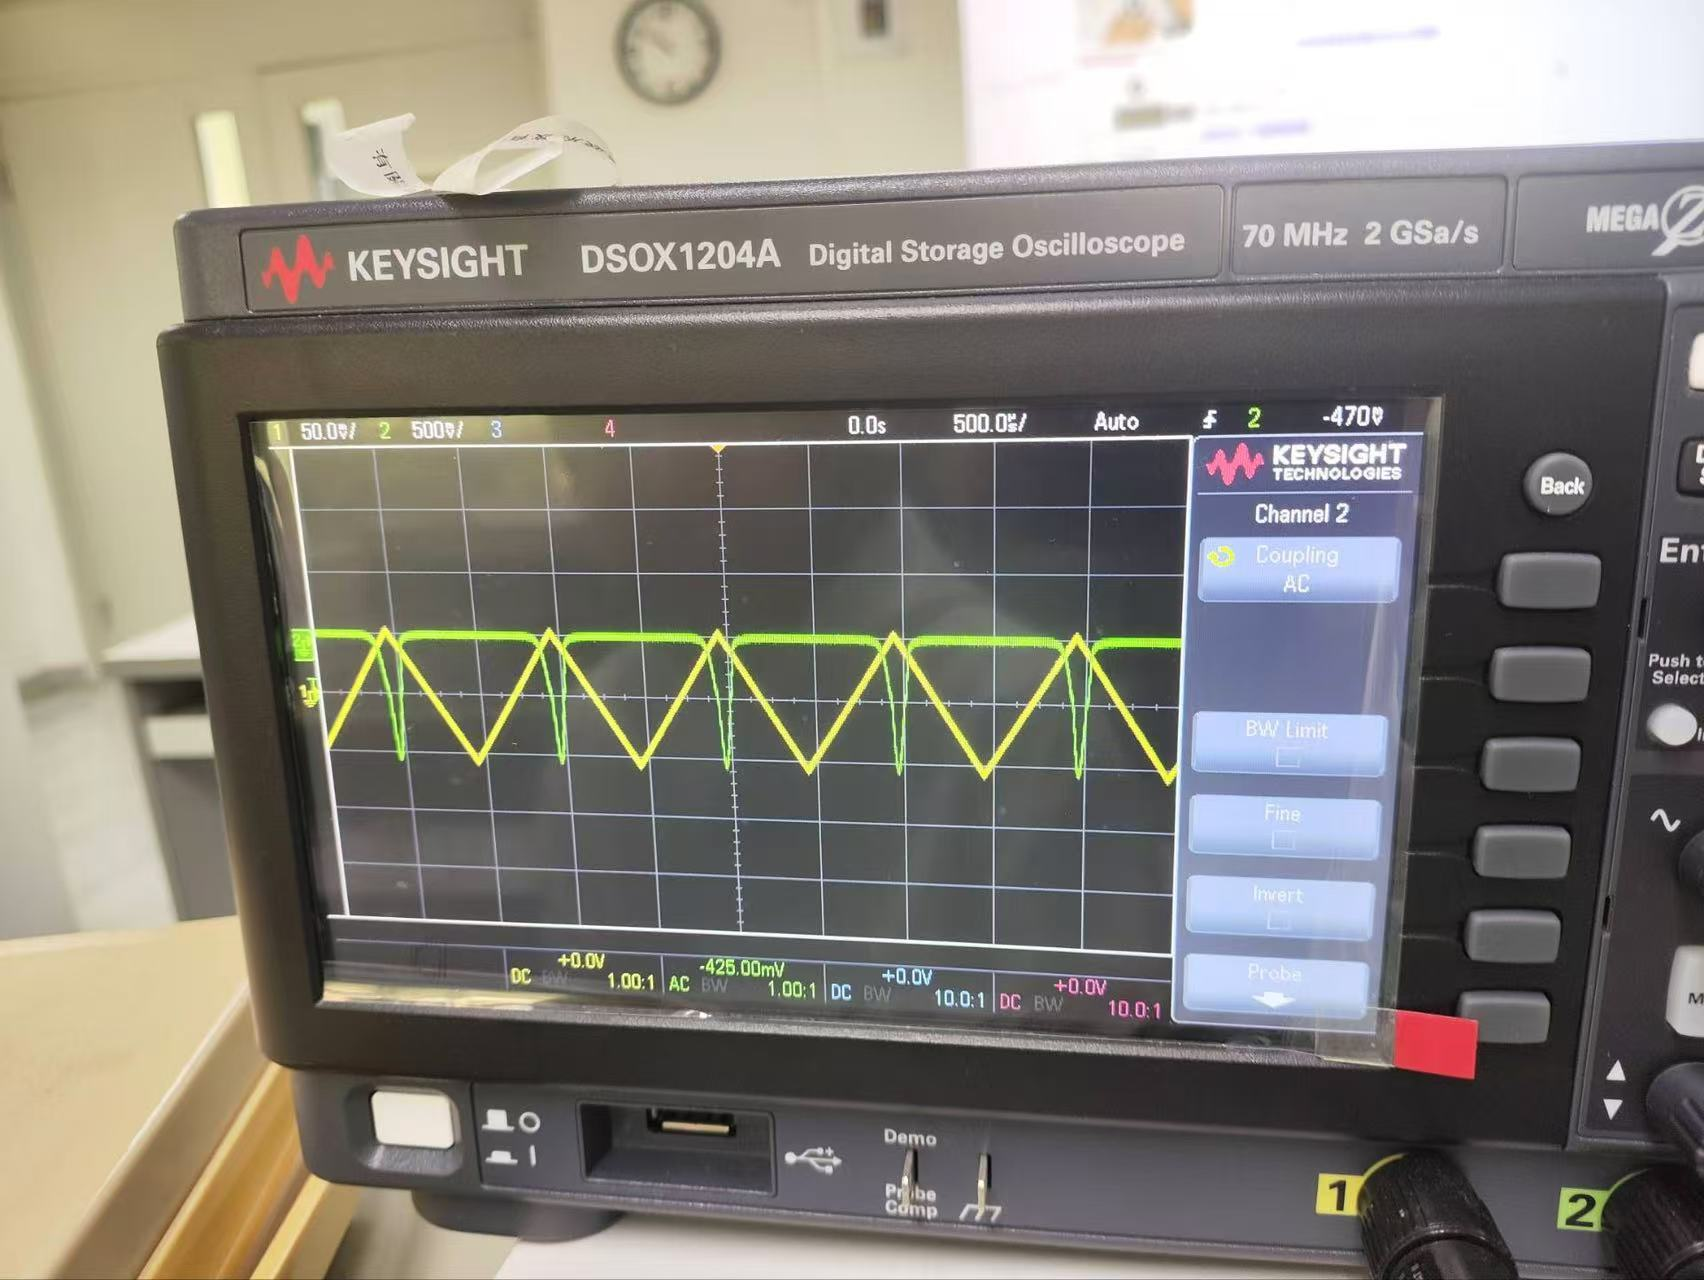
\includegraphics[width=0.5\linewidth]{Lab11/l11dwf.jpg}
    \caption{Wavefrom}
    \label{l11dwf}
\end{figure}
\FloatBarrier
        The amplitude of $v_i$ we adjusted is 0.530V. 
    \end{itemize}
    
\section{Discussion}
This experiment is conducting under the condition of using multiple combined resistors, this might cause the inaccuracy of the resistance.\par
Some of plots are missing in this experiment report. 

\section{Conclusion}
In this experiment, we verified multiple operational amplifier circuits, these circuits were designed with various purposes. And these circuits performed expected results which very close to the results of theoretical relationship we predicted.\par
These circuits strengthen my knowledge of the operational amplifiers' practical usage.\par
In summary, these experiments reinforce my theoretical concepts while emphasizing practical considerations.